\chapter{État de l'Art}

\section{Introduction}

L'étude des données spatio-temporelles a connu un réel essor ces dernières années. En effet, avec les volumes croissants de données urbanistiques recensées et rendues disponibles, des nouvelles opportunités se sont créées pour l'analyse de données avec pour idée d'améliorer la vie des citoyens au travers de prises de décisions politiques basées sur des faits. Il s'agit donc essentiellement de méthodes de régression et de prédictions.

Cet état de l'art est inspiré par le livre \textit{Statistics for spatio-temporal data}, écrit par Noel Cressie et Christopher K. Wikle~\cite{cressie2015statistics}. Ceux-ci proposent une vision très étendue de tous les aspects statistiques qui rentrent en compte tant dans les processus de modélisation que dans les techniques employées dans ce vaste champ de l'informatique. Ainsi que de \textit{Handbook of spatial Statistics} de Alan E. Gelfand, Peter J. Diggle, Montserrat Fuentes et Peter Guttorp~\cite{gelfand2010handbook} qui offrent un point de vue plus pratique aux travers des techniques et études sur le sujet.

\section{Spatial processes}

\subsection{Introduction}\label{SpatialProcesses}

Dans les problèmes liés à l'espace, les données sont rarement indépendantes entre-elles et, donc, certaines techniques standards qui font appels à l'indépendance des variables deviennent caduques dans ce domaine~\cite{de2010spatial}. La dépendance spatiale se traduit par une covariation des propriétés, les caractéristiques et propriétés des lieux proches ont tendance à être plus corrélés tant positivement que négativement que des points fort éloignés. Ce phénomène d'auto-corrélation (non-indépendance des variables) viole des conditions d'application de techniques statistiques classiques~\cite{legendre1993spatial}.

Très naturellement, afin de mieux percevoir les effets locaux, on définit des notions de proximités (d'auto-corrélation spatiale) tant au niveau des distances (\textit{Ripley's K/L-function})~\cite{dixon2002ripley} que des individus (\textit{Moran's I global \& Geary's C local})~\cite{f2007methods}.

Il y a trois branches majeures dans l'analyse spatiale statistique~\cite{gelfand2010handbook}:
\begin{itemize}
    \item variation continue (\textit{continuous spatial variation})$^{[\ref{Variation_continue}]}$, axée sur la prédiction;
    \item variation discrète (\textit{discrete spatial variation})$^{[\ref{Variation_discrete}]}$, axée sur l'inférence et les interactions entre les données;
    \item processus ponctuels (\textit{spatial point processes})$^{[\ref{Variation_ponctuelle}]}$, axée sur l'inférence et la positions des points par eux-mêmes;
\end{itemize}

On attribue à Julian Besag des modèles et méthodes d'inférence pour analyser des données discrètes (sur des \textit{lattices})~\cite{besag1974spatial}. À Brian Ripley, des approches systématiques pour des processus à point spatial~\cite{ripley1977modelling}. Les variations spatiales continues sont quant à elles plus anciennes et peuvent être associées aux travaux de Danie G. Krige~\cite{cressie1990origins} et Georges Matheron~\cite{matheron1973intrinsic}.

Le modèle géostatistique le plus classique (ou le plus général) décompose le processus aléatoire comme suit:

\begin{equation}
    Z(s) = Y(s) + \epsilon(s)
\end{equation}

avec $Y(s)$ le processus stochastique en fonction de la position $s$, $Z(s)$ l'observation liée et $\epsilon(s)$ l'erreur (de mesure, par exemple) associée.

\subsection{Variation continue}\label{Variation_continue}

Lorsqu'on aborde la notion d'espace, il est normal de penser tout d'abord à des variables continues a l'instar de la géométrie différentielle et son analyse vectorielle. Naturellement, plusieurs modèles de probabilité liés aux espaces (ayant $d$ dimensions) ont fait leur apparition et bon nombre considèrent une définition de processus stochastiques très génériques:

\begin{equation}
    \{ Y(s) : s \in D_{s} \subset \mathbb{R}^{d} \}
\end{equation}

avec l'idée qu'à chaque position est associée une probabilité $\omega \in \Omega$. Ce processus est valide si la distribution jointe est bien définie et consistante (par permutation des éléments et marginalisation notamment)~\cite{kolmogorov1960strong}.

En outre, il est important de faire mention de deux définitions:
\begin{itemize}
    \item On qualifie un processus stochastique de "strictement stationnaire" si les lois de probabilités sont invariantes par translation. Les probabilités jointes ne sont pas modifiées si on déplace toutes les positions par un vecteur $h$.
    \item Et de "stationnaire du second-ordre (ou faible)" si le processus satisfait ces deux propriétés:
    
    \begin{equation}
        \mathbb{E}(Y(s)) = \mathbb{E}(Y(s + h)) = \mu
    \end{equation}
    et
    
    \begin{equation}
        cov(Y(s), Y(s + h)) = cov(Y(0), Y(h)) = C_{Y}(h)
    \end{equation}
    
    où $C_{Y}(h)$ est la fonction de covariance. La matrice de covariance est souvent inconnue et l'exprimer purement en terme de distance permet de diminuer le nombre de dimensions afin de plus facilement pouvoir l'estimer.
\end{itemize}

Remarquons que la stationnarité du second ordre implique celle stricte pour les modèles gaussiens. D'autre part, sous l'hypothèse du second ordre, Mathéron a proposé la définition d'une fonction ($f: \mathbb{R}^{+} \rightarrow \mathbb{R}$) dénommée semi-variogramme~\cite{matheron1971theory}, plus connue sous sa forme forte comme le \textit{semi-variogramme de Matérn}:

\begin{equation}
    \gamma_{Y}(h) = \frac{1}{2} var(Y(s + h) - Y(s)) = C_{Y}(0) - C_{Y}(h)
\end{equation}

Les variogrammes sont une classe de fonctions très importantes dans la théorie du \textit{kriging}$^{[\ref{Kriging}]}$, elles sont définies par la manière dont les observations évoluent entre deux positions et sont donc par nature aléatoire; les semi-variogrammes sont ces fonctions divisées par deux. Ils mesurent le degré de dépendance spatiale. Dans le cas stationnaire, les variogrammes ne dépendent que de la distance $h$ alors que les fonctions de covariance ne le deviennent qu'à partir du second ordre. De plus, l'estimation du variogramme n'est pas biaisée par la moyenne, au contraire de la covariance. Toutefois, tout variogramme respectant la condition de matrice définie non-positive peut être employé~\cite{ver1993multivariable}.

Un variogramme peut être qualifié d'"isotropique" s'il peut être écrit sous la forme d'une fonction de $\| h \|$ et lorsqu'on prend en considération un modèle muni d'un norme $L^{2}$ (distance euclidienne), les variogrammes peuvent montrer une discontinuité près de l'origine, on parle alors de \textit{nugget effect}~\cite{cressie2015statistics}. Sa qualité peut être mesurée par le biais des techniques liées au \textit{Goodness of Fit}~\cite{diggle2013statistical}. Lorsque le modèle n'est pas isotropique, on peut l'approcher par un isotropique associé à une transformation linéaire.

\subsection{Kriging}\label{Kriging}

Le \textit{kriging} (ou krigeage) est une méthode d'estimation linéaire optimale non-biaisé qui minimise la variance (\textit{BLUE}), sous les hypothèses de Gauss-Markov. Il s'agit d'une méthode des moindres carrés ordinaire (\textit{OLS}). Il tient compte non seulement de la distance entre les données et le point d'estimation, mais également des distances entre les données deux-à-deux. L'idée fondamentale est de prédire la valeur de la fonction en un point comme une somme pondérée des valeurs connues et avoisinantes à celui-ci. Le \textit{kriging} en lui-même est un nom générique pour une méthodologie afin de construire un estimateur; en effet, plusieurs techniques existent en vue de satisfaire certains critères sous base de présomptions sur le modèle. Son principal avantage est qu'il permet d'obtenir l'erreur sur l'estimation~\cite{cressie1990origins}.

\begin{equation}
    \hat{Y}(s_{0}) = \sum_{i = 1}^{n} l_{i} Z(s_{i}) + k = l'Z + k
\end{equation}
où $s_{0} \in D_{s}$ est la position de la prédiction et $s_{i}$ sont les observations (au nombre de $n$). Tout en minimisant la variance de la prédiction (\textit{Mean Square Prediction Error}):
% We do that because it ignores the data model and implicitely assumes that \sigma_{e}^{2} = 0
\begin{equation}
    MSPE(l, k) = var(Y(s_{0}) - l'Z - k) + \mathbb{E}(Y(s_{0}) - \hat{Y}(s_{0}))^{2}
\end{equation}

\begin{itemize}
    \item Le \textit{simple kriging} est sans doute le plus facile mathématiquement. Il fait l'hypothèse d'une moyenne constante, estimée par la moyenne de l'échantillon des données, et d'une covariance connue. Il peut être interpréter comme la tendance générale des données corrigée par la covariance locale des données.
    \begin{equation}
        \hat{Y}(s_{0}) = \mu_{Y}(s_{0}) + cov(Y(s_{0}), Z)'C_{Z}^{-1}(Z - \mu_{Y})
    \end{equation}
    Avec pour variance:
    \begin{equation}
        \sigma_{Y, simp.krig.}^{2}(s_{0}) = MSPE(\hat{l'}, \hat{k}) = C_{Y}(s_{0}, s_{0}) - cov(Y(s_{0}), Z)'C_{Z}^{-1}cov(Y(s_{0}), Z)
    \end{equation}
    \item L'\textit{ordinary kriging} remplace la moyenne de l'échantillon par l'estimation des moindres carrés de celle-ci.
    \item L'\textit{universal kriging} substitue la moyenne constante par un modèle de régression; il est le plus employé mais introduit beaucoup de difficultés techniques mathématiquement et se décline en de nombreuses formes pour des cas spéciaux (valeurs binaires, valeurs discrètes, ...)~\cite{matheron1971theory}.
\end{itemize}

Il existe des modèles connexes qui ne prennent pas en compte l'hypothèse de stationnarité (indépendance entre l'observation et le lieu considéré) suite aux résultats des tests de \textit{Moran's I} ou de "Breusch-Pagan"~\cite{breusch1979simple}. Les deux autres grandes familles de modèles sont les \textit{Spatial autoregressive model} (SAR) à l'instar des séries temporelles$^{[\ref{AR}]}$ et \textit{Geographically Weighted Regression} (GWR régression locale sur un modèle) qui prennent en compte les phénomènes spatiaux~\cite{gelfand2010handbook}.

Exemple de \textit{kriging} en R, où on essaye de prédire la position de gisements de zinc le long de la Meuse en fonction de sites connus et de leur concentration:

\lstset{basicstyle=\scriptsize}
\lstinputlisting[language=Python]{Kriging/Kriging.R}

\begin{figure}[!htb]
\minipage{0.32\textwidth}
  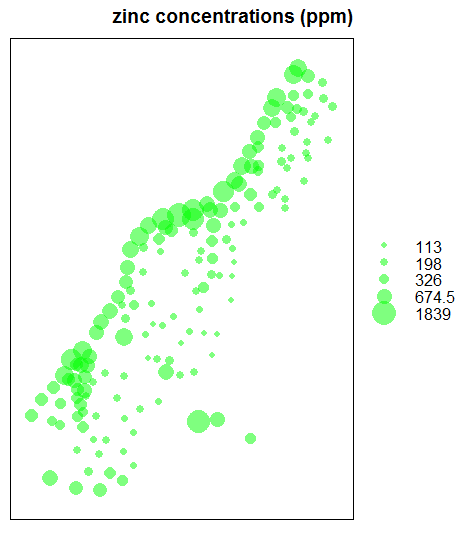
\includegraphics[width=\linewidth]{EtatDeLArt/Kriging/ZincConcentrations.png}
\endminipage\hfill
\minipage{0.32\textwidth}
  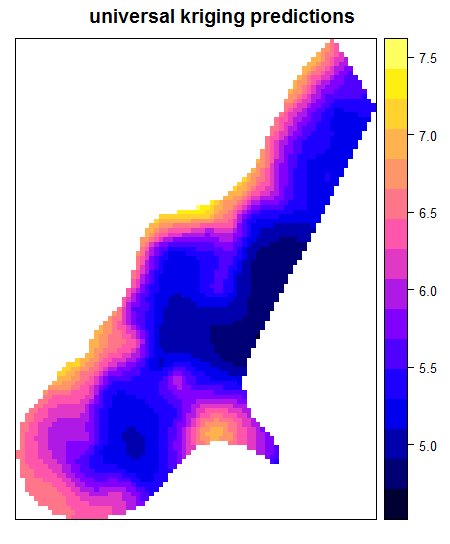
\includegraphics[width=\linewidth]{EtatDeLArt/Kriging/UniversalPredictions.png}
\endminipage\hfill
\minipage{0.32\textwidth}%
  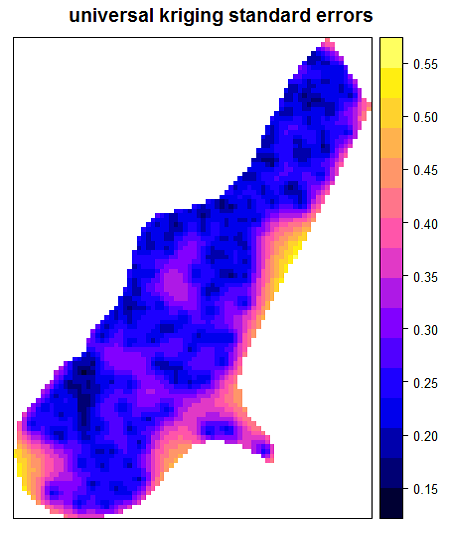
\includegraphics[width=\linewidth]{EtatDeLArt/Kriging/UniversalErrors.png}
\endminipage
\end{figure}

Librairies R associées: sp (classes et méthodes pour les données spatiales)~\cite{sppackage}, gstat (variogramme et \textit{kriging})~\cite{pebesma2004multivariable}, spacetime (axée données spatio-temporelles)~\cite{pebesma2012spacetime} ou geoR (outils standards d'analyse géostatistque)~\cite{geoRpackage}.

\subsection{\textit{Lattice} \& MRF}\label{Variation_discrete}

L'hypothèse d'un modèle continu n'est pas toujours nécessaire, il est parfois suffisant de travailler avec un sous-ensemble fini, discret, un treillis (\textit{lattice graph}). Typiquement, une grille composée de petits rectangles. Ce procédé nécessite d'introduire une notion de distance au travers d'une matrice souvent notée $W$ et dont l'entrée $(i, j)$ correspond à la distance entre $i$ et $j$.

Une modélisation statistique sur base d'une collection finies de variables est souvent envisagée sous la forme des champs aléatoires de Markov (\textit{Markov Random Field}). L'idée était de généraliser le concept des processus de Markov à d'autres dimensions tout en incluant la notion de dépendance~\cite{besag1974spatial}. Un MRF est un moyen simple de représenter des distributions conditionnelles. Ceci permet de s'intéresser à une variable à la fois tout en simplifiant la simulation. Le concept clef est qu'au lieu de s'intéresser à l'instant $t$ connaissant les $t - 1, t - 2, ...$, comme pour les processus de Markov (ce qui nécessite de définir une notion d'ordre), on regarde les positions voisines comme "historique" de la fonction~\cite{zhang2001segmentation}.

\begin{equation}
    Y(s_{i})|Y_{-i} = Y(s_{i})|Y(N(s_{i})) ~~ \forall i \in D_{s} \subset \mathbb{R}^{d}
\end{equation}

avec $N(s_{i})$ l'ensemble des voisins du point $s_{i}$ et $_{-i}$, tous les points exceptés $i$; on cherche à exprimer $Y(s_{i})$ connaissant son voisinage ($.|Y(N(s_{i}))$).

Les probabilités conditionnelles définissent notre MRF, seulement nous préférerions trouver les probabilités jointes associées afin de pouvoir appliquer de puissants théorèmes (Hammersley–Clifford~\cite{grimmett1973theorem} ou le résultat des Geman~\cite{geman1984stochastic}) afin de ne plus être contraint à un ensemble de points fixés. Kaiser \& Cressie donnent une procédure afin de calculer ces dites probabilités sous des hypothèses suffisamment généralistes~\cite{kaiser2000construction}.

Quelques modèles existent en rapport avec ces notions employant des distributions diverses. Citons les modèles dits "auto Poisson", "auto logistique", "auto binomial" ou "auto Beta"~\cite{west1985dynamic, lichstein2002spatial}. Mais le plus classique est sans doute l'"auto Gaussien".

Le modèle CAR (\textit{conditional autoregressive}) est défini par une distribution gaussienne:
\begin{equation}
    \mathbb{P}(y(s_{i}) | y(N(s_{i}))) = (2\pi\tau_{i}^{2})^{-1/2} exp[-(y(s_{i}) - \theta_{i})^{2} / 2\tau_{i}^{2})]
\end{equation}
où $\tau_{i}^{2}$ est la variance conditionnelle et $\theta_{i}$ est interprété comme une moyenne, fonction du voisinage du point, corrigée par la variance locale:
\begin{equation}
    \theta_{i}(y(N(s_{i}))) = E(Y(s_{i}) ~ | ~ y(N(s_{i}))) = \mu(s_{i}) + \sum\limits_{s_{j} \in N(s_{i})} c_{ij} (y(s_{j}) - \mu(s_{j}))
\end{equation}

Delà, on peut définir la matrice $C$ de covariance avec les coefficients $c_{ij} = c_{ji}$ et $M$ diagonale avec les valeurs de $\tau_{i}^{2}$, on obtient alors une expression symétrique, définie positive qui permet d'obtenir la distribution jointe gaussienne~\cite{besag1974spatial}:

\begin{equation}
    Y \thicksim Gau(\mu, (I - C)^{-1}M)
\end{equation}

CAR est plus approprié aux situations où la dépendance est du premier ordre, où l'auto-corrélation locale est forte tandis que SAR$^{[\ref{AR}]}$ est adapté au second ordre et à une auto-corrélation plus globale. Cependant, l'interprétation de ces modèles n'est pas forcément intuitive. Les modèles SAR sont bien estimés par \textit{maximum likelihood} mais absolument pas par MCMC (lié à la difficulté d'introduire des effets aléatoires au contraire du modèle CAR)~\cite{wall2004close}.

Librairies R associées: CARBayes (modèles CAR)~\cite{CarBayes}, spdep (permet de définir des métriques et d'utiliser SAR)~\cite{spdep} ou spBayes (modèles bayésiens pour les problèmes spatio-temporels liés aux \textit{lattice})~\cite{finley2007spbayes}.

\subsection{Spatial Point Process}\label{Variation_ponctuelle}

Sous ce nom, on sous-entend un processus aléatoire dont les réalisations consistent en un ensemble fini ou dénombrable de points dans un espace. Un exemple serait la répartition des arbres dans une forêt. On tend à définir le processus $Z$ tel que $Z(A)$ dénote le nombre d'événements survenus dans une région $A \subset D_{s} \subset \mathbb{R}^{d}$ dite "Lebesgue mesurable"~\cite{daley2007introduction}.

Intuitivement, la notion de Poisson semble bien correspondre à la description du problème, estimer le nombre d'évènements dans un intervalle. Seulement, on ne connaît pas le paramètre de la distribution associée à une région, qui serait une indication sur le nombre d'occurrences. Il faut donc créer une fonction "d'intensité" qui dépend de la position et qui représente le potentiel d'apparition en vue d'obtenir le nombre d'événements dans cet intervalle. On définit la fonction d'intensité du premier ordre comme suit (en relation avec le théorème de Campbell)~\cite{baddeley2007spatial}:

\begin{equation}
    \lambda(s) = \lim_{|ds| \to 0} E(Z(ds))) / |ds| ~~ \forall s \in D_{s} \sim E(Z(A)) = \int_{A} \lambda(s) ds ~~ \forall A \subset D_{s}
\end{equation}

Dans le contexte spatial, on parle souvent de processus de Cox qui est une généralisation de Poisson dans lequel la moyenne n'est pas constante mais varie avec l'espace ou le temps~\cite{cox1955some}. On peut étendre ce modèle en introduisant une notion analogue à la covariance, mais pour la fonction d'intensité, ainsi que l'équivalent des variogrammes (\textit{K-functions}). Une autre famille très populaire est celle de Gibbs qui est équivalent à la notion de \textit{Markov point process} et trouve son origine dans la physique. Le but est de modéliser un ensemble de points où certaines propriétés physiques (notamment d'attraction-répulsion) sont respectées. Mathématiquement, c'est loin d'être trivial, il faut créer une fonction de potentiel qui permet de minimiser les probabilités que deux points soient situées l'un à côté de l'autre. La simulation s'effectue par le biais d'un \textit{MCMC}~\cite{illian2008statistical}.

Librairies R associées: spatstat (incroyablement riche pour étudier les problèmes ponctuels)~\cite{baddeley2016spatial}, lgcp (pour les processus de Cox)~\cite{lgcp} ou PtProcess (analyse plus orientée sur l'aspect temporelle)~\cite{ptprocess}.

\section{Processus temporel}

\subsection{Introduction}

Lorsqu'on se trouve face à des données récoltées, il n'est pas rare de définir et catégoriser les événements selon une notion d'ordre temporel. En effet, certaines observations sont fonction du temps et il peut être utile de voir si l'aspect temporel occupe une part importante dans l'analyse de ces données~\cite{kendall1946advanced}.

On définit les modèles temporaux de manière très générique:

\begin{equation}
    \{ Y(t) : t \in D_{t} \}
\end{equation}

Traditionnellement, on décompose ces phénomènes en quatre éléments: les tendances (changements dans la moyenne à long terme), les variations saisonnières, les cycles (hebdomadaires ou pluriannuels) et les fluctuations irrégulières afin d'avoir une meilleure flexibilité au niveau de la modélisation. Il n'est pas rare non plus de considérer des phénomènes dits stationnaires où les premiers moments restent constants. Les définitions sont analogues aux processus spatiaux$^{[\ref{Variation_continue}]}$ mais le temps remplace la notion d'espace~\cite{chatfield2000time}. 

Pendant longtemps, on a employé des modèles purement déterministes liés aux équations aux différences ou différentielles, mais ceux-ci semblent mener, en pratique, à des résultats souvent inférieurs aux modèles stochastiques qui se basent sur les notions de bruit blanc ou de marche aléatoire (\textit{random-walk})~\cite{chatfield2016analysis}.

\subsection{Processus auto-régressif}\label{AR}

Il n'est pas rare qu'une observation soit dépendante d'une ou plusieurs précédentes. On modélise ce genre de comportement par des processus ayant la propriété d'être auto-régressif. La taille de l'historique de la fonction définit son ordre.

\begin{equation}
    AR(p) \equiv Y_{t} = \alpha_{1} Y_{t - 1} + ... + \alpha_{p} Y_{t - p} + \epsilon_{t}
\end{equation}

avec $ \epsilon_{t} $ est un processus de bruit blanc et $\alpha_{k}$ des constantes. Remarquons que le cas AR(1) correspond à la série géométrique (si $|a_{k}| < 1$). Seulement, il est souvent préférable de définir une valeur moyenne locale afin d'être en mesure de décrire l'erreur comme une combinaison de celle présente et passée. On a alors une fenêtre coulissante définissant une moyenne locale, le \textit{moving average}~\cite{shumway2010time}:

\begin{equation}
    MA(q) \equiv Y_{t} = W_{t} + \beta_{1} W_{t - 1} + ... + + \beta_{q} \epsilon_{t - q}
\end{equation}

avec $\epsilon_{t}$ des variables aléatoires (bruit blanc) et $\beta_{k}$ des constante. L'estimation de ces paramètres n'est pas aisée et on emploie souvent les équations de Yule-Walker et l'algorithme de Durbin-Levinson. Lorsqu'on combine ces deux notions, nous obtenons le modèle \textit{ARMA} qui est à l'origine de bon nombre de variantes, notamment du \textit{ARIMA} qui permet de gérer les cas non-stationnaires en effectuant récursivement la différence entre les données $t$ et $t+1$ "$d$ fois" (terme d'"intégration" I(d))~\cite{box2015time}. Dans le cadre multivarié, ce modèle est étendu pour donner naissance à \textit{VAR} et ses dérivés mais il peut parfois effectuer de l'overfitting et l'on préfèrera alors employé un \textit{BVAR}~\cite{lutkepohl2005new}.

Seulement, comment trouver les bons paramètres pour modéliser notre problème. Il faut d'abord se poser la question de la stationnarité par le biais du test de Dickey-Fuller. Ensuite, avons-nous affaire à un phénomène plutôt de type AR ou MA et quels sont leurs ordres ? AR donne des effets plus longs dans la durée parce que son auto-corrélation décline peu à peu tandis que MA en donne des brefs. On peut se baser sur le \text{lag} de l'auto-corrélation qui tend vers zéro au bout de $q$ étapes pour le MA(q). Le côté AR(p) est plus difficile, on se base sur la valeur à partir de laquelle elle devient négligeable au bout de $p$ étapes dans les \textit{partial auto-correlation function}. Enfin, le terme d'intégration I(d) est évalué en regardant quand la tendance générale disparaît. Bien sûr, on peut augmenter les paramètres petit à petit et étudier l'évolution du maximum de vraisemblance~\cite{chatfield2016analysis}.

Lorsqu'on veut réaliser des prédictions, on peut employer les méthodes mentionnées ci-dessus, mais également, le \textit{exponential smoothing} qui consiste simplement à appliquer une régression par des fonctions (exponentielles ou polynomiales), le fameux filtre de Kalman$^{[\ref{FiltreKalman}]}$ ou encore des modèles bayésiens~\cite{shumway2010time}.

\subsection{Représentation Spectrale}

Très logiquement, il est normal de vouloir observer les phénomènes temporaux dans le domaine des fréquences. La notion d'auto-covariance est complétée par celle de périodogramme qui donne des indications sur les harmonies. Il ne reste plus qu'à calibrer les coefficients spectraux avec des techniques classiques (à l'instar de l'\textit{exponential smoothing}). Un des grands avantages de cette représentation est qu'il devient facile de comparer deux séries temporelles afin de voir si elles sont corrélées. L'idée est de considérer une des séries comme l'entrée et l'autre comme la sortie pour trouver les propriétés du système linéaire qui pourrait y être associé~\cite{box2015time}.

Exemple de prédiction avec un modèle ARIMA, sur base du nombre de voyageurs prenant l'avion chaque mois:

\lstset{basicstyle=\scriptsize}
\lstinputlisting[language=Python]{AR/AR.R}

\begin{figure}[!htb]
\minipage{0.5\textwidth}
  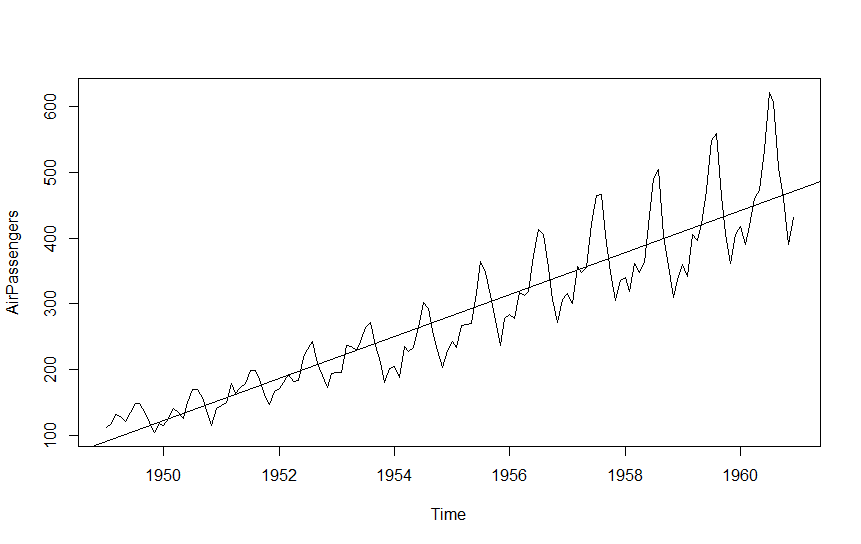
\includegraphics[width=\linewidth]{EtatDeLArt/AR/DataAirPassengers.png}
\endminipage\hfill
\minipage{0.5\textwidth}
  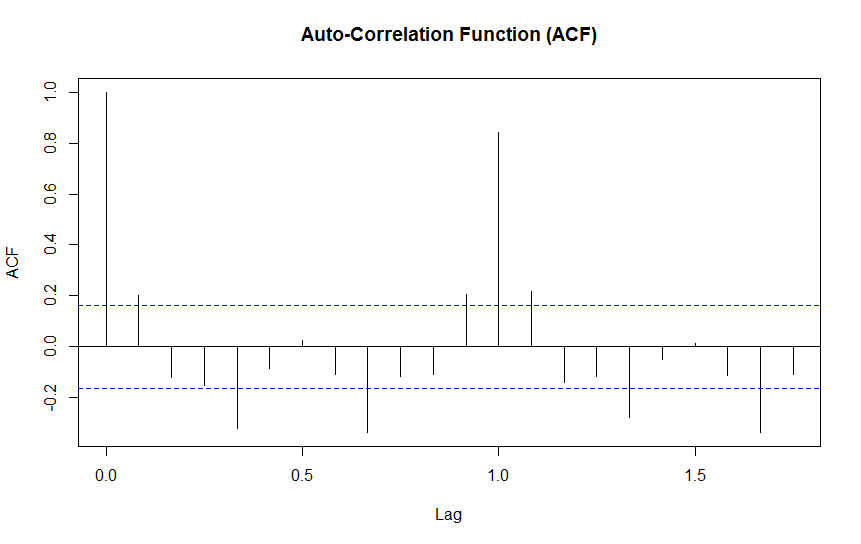
\includegraphics[width=\linewidth]{EtatDeLArt/AR/ACF.png}
\endminipage\hfill

\minipage{0.5\textwidth}
  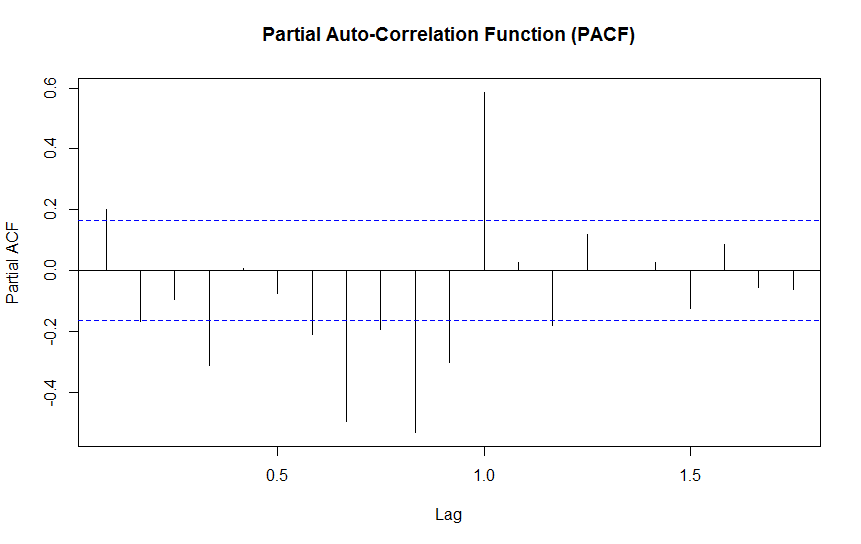
\includegraphics[width=\linewidth]{EtatDeLArt/AR/PACF.png}
\endminipage\hfill
\minipage{0.5\textwidth}
  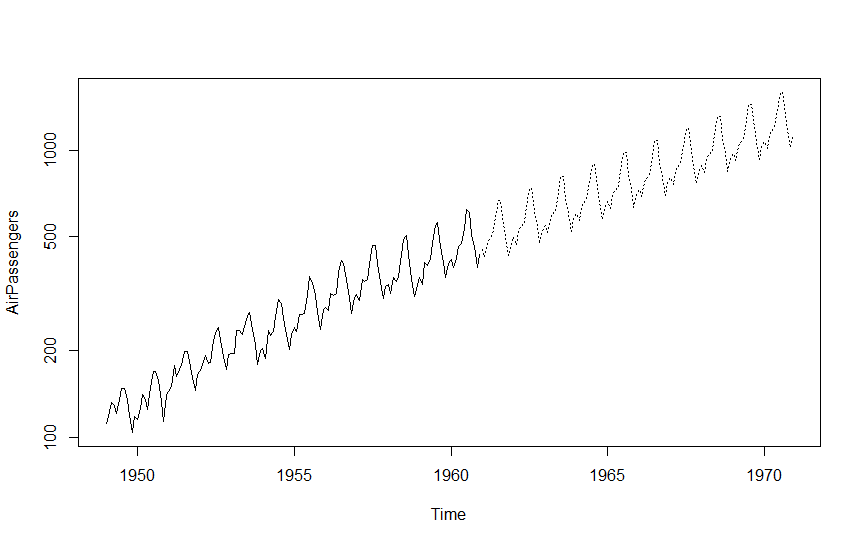
\includegraphics[width=\linewidth]{EtatDeLArt/AR/Prediction.png}
\endminipage\hfill

\center{Illustrations des différentes notions pour la prédiction du nombre de passagers.}
\end{figure}

Librairies R associées: timeSeries (modèles pour les séries temporelles financielles)~\cite{timeSeries}, forecast (ensemble de modèles prédictifs)~\cite{forecast} ou AnomalyDetection (pour trouver des anomalies parmi les saisons)~\cite{twitter-anomaly-detection-2015}.

\section{Processu spatio-temporel}

\subsection{Introduction}

Les processus spatio-temporels combinent les notions liées aux sections précédentes afin de décrire un modèle sur de larges intervalles de temps et d'espace. Les objectifs sont nombreux: effectuer des prédictions dans le temps ou dans l'espace, inférer les comportements sur base des observations et tenter d'approcher ces processus par des modèles.

Un processus spatio-temporel est défini de manière très générale:

\begin{equation}
    \{ Y(s, t): (s, t) \in D_{s} \times D_{t} \subset \mathbb{R}^{d} \times \mathbb{R} \}
\end{equation}

avec l'idée sous-jacente que les valeurs sont dépendantes du voisinage et du passé.

Bien sûr, on peut envisager le problème sous la forme d'un système d'équations différentielles, mais ce modèle théorique est souvent inconnu et difficile à aborder~\cite{gelfand2010handbook}.

\subsection{Fonctions de covariance}

Comme les solutions analytiques sont difficiles à appréhender, il vaut mieux décrire le processus par un modèle statistique:

\begin{equation}
    Y(s, t) = \mu(s, t) + \beta(s) + \gamma(t) + \kappa(s, t) + \delta(s, t) ~~ (s, t) \in D_{s} \times D_{t}
\end{equation}

avec: $\mu(s, t)$ une moyenne déterministe, $\beta(s)$ la variation commune des endroits à travers le temps, $\gamma(t)$ du temps pour les positions, $\kappa(s, t)$ variation sur le modèle de $\mu$ et $\delta(s, t)$ le bruit (le \textit{nugget effect}). De surcroît, on fait l'hypothèse de la description sur base des deux premiers moments~\cite{wikle2003bf}.

A l'instar des processus spatiaux$^{[\ref{Variation_continue}]}$, les notions de covariance jouent un rôle clef. Une propriété importante est le fait que la fonction soit définie non-négative, ce qui permet d'appliquer le théorème de Bochner~\cite{cressie1999classes} et de parler de son spectre~\cite{stein2012interpolation}. De même, il est intéressant d'avoir une certaine stationnarité tant spatiale que temporelle. Et on parle de fonction de covariance spatio-temporelle séparable lorsqu'on peut séparer les deux notions de covariance comme suit:

\begin{equation}
    cov(Y(s, t), Y(x, r)) = C^{(s)}(s, x) . C^{(t)}(t, r)
\end{equation}

Cette hypothèse de séparabilité simplifie la construction de modèles, diminue le nombre paramètres et facilite les calculs (inversion de matrices) aux dépens des interactions spatio-temporelles (très présentes en physique)~\cite{genton2007separable}. Cette séparabilité implique la notion de symétrie complète ($C(s, t) = C(s, -t) = C(-s, t) = C(-s, -t)$) et peut être testée~\cite{fuentes2006testing}. Réciproquement, le cas inséparable a également été fortement étudié~\cite{fuentes2008class}.

\subsection{Kriging spatio-temporel}

Les fonctions de covariance n'ont jamais qu'un rôle descriptif et, malgré leur souplesse, il est difficile de se rendre compte de l'étiologie du processus. Seulement, elles jouent un rôle dans la technique du \textit{kriging} qui se base sur la définition de variogrammes. Or le \textit{kriging} ne nécessite pas la notion de stationnarité pour exister~\cite{cressie1986kriging}. On peut alors étendre le \textit{kriging} aux données spatio-temporelles. En supposant que les données soient de la forme:

\begin{equation}
    Z(s_{i}, t_{ij}) = Y(s_{i}, t_{ij}) + \epsilon(s_{i}, t_{ij}) ~~ i \in S, j \in T_{i}
\end{equation}

où $S$ représente l'ensemble des positions et $T_{i}$ les observations associé à l'endroit $i$ (par rapport au temps).

Le \textit{simple kriging} revient alors à optimiser l'expression suivante:

\begin{equation}
    \hat{Y}(s_{0}, t_{0}) \equiv \sum_{i=1}^{n}\sum_{j=1}^{T_{i}} l_{ij}Z(s_{i}, t_{ij}) + k \equiv l'Z + k
\end{equation}

sous minimisation de l'expression:

\begin{equation}
    E(Y(s_{0}, t_{0}) - l'Z - k)^{2}
\end{equation}

Cette technique nécessite que la moyenne soit connue. Si elle est supposée constante, elle donne naissance à l'\textit{ordinary kriging} et si elle est combinaison linéaire, on parle de \textit{universal kriging}~\cite{ver1993multivariable}.

Généralement, on préfère parler de \textit{cokriging} qui est une extension multivariée de ce concept et qui prend en compte, non seulement l'information des mesures directes, mais également des autres composantes. Dans le but de fournir un meilleur estimateur, moins sujet à de grandes variations car étayées par les autres observations. Ainsi améliorer les prédictions des variables spatiales trop peu échantillonnées en exploitant davantage la corrélation spatiale attachée à d'autres variables plus facilement mesurables~\cite{wackernagel2013multivariate}.

\subsection{Séries temporelles}

Il y a deux grandes familles de séries temporelles liées aux données spatio-temporelles, celle liée aux processus géostatistiques et celle des \textit{lattice}. Dans les deux cas, la temps est vu de manière discrète et les processus spatiaux deviennent multivariés afin de compenser cette perte temporelle~\cite{rouhani1990multivariate}.

Pour les processus spatiaux continus, l'idée est d'exprimer le résultat à l'instant $t$ en un lieu comme une fonction (potentiellement non linéaire) de l'instant $t - 1$:

\begin{equation}
    Y_{t}(s) = \mathcal{M}(s, Y_{t-1}(.)) + \epsilon_{t}(s) ~\text{avec}~ \mathcal{M}(s, f(.)) \equiv \int_{\mathbb{R}^{d}} m(s, x)f(x) dx
\end{equation}

avec $f(.) \in \mathbb{R}^{d}$ une fonction quelconque telle que l'intégrale existe et $m(s, x)$ qui contrôle l'influence de $Y_{t-1}$ sur l'instant actuel. Cette forme est liée au filtre de Kalman, offre beaucoup de flexibilité et possède de bonnes propriétés, notamment pour la réduction de dimensions ou la représentation de modèles spatiaux statiques~\cite{wikle1999dimension}.

Dans le cas des \textit{lattice}, on voit le problème sous un autre angle. À un instant $t$, toutes les valeurs aux différentes positions représentent un élément de la série temporelle n-variée (une dépendance par rapport au temps étant plus naturelle). On emploie alors des modèles de type SAR ou CAR~\cite{allcroft2003latent}. Ou, ce qui est plus classique pour les séries temporelles, la notion de modèle à vecteur autorégressif (VAR) qui est employé pour capturer les interdépendances linéaires parmi les multiples séries temporelles. La notion de VAR vise à simplifier celle de \textit{Spatio-Temporal AutoRegressive Moving-Average} (STARMA) en limitant le nombre de paramètres~\cite{pfeifer1980identification}.

\subsection{Modèles hiérarchiques dynamiques spatio-temporels}

Les processus spatio-temporels sont de nature à être modéliser par des dynamiques, on parle alors de \textit{dynamical spatio-temporal models} ou DTSM. Or, ces processus sont difficile à appréhender et on tente alors de simplifier en reformulant le problème comme suit~\cite{wikle1998hierarchical}:

\begin{tabular}{ll}

    $\text{Data model}:$ & $ \lbrack data|process, parameters\rbrack $ \\
    $\text{Process Model}:$ & $ \lbrack process|parameters\rbrack $ \\
    $\text{Parameter Model}:$ & $ \lbrack parameters\rbrack $ \\
    \\
    $ \lbrack process, parameters|data \rbrack $ & $\propto \lbrack data|process, parameters\rbrack $ \\
    & $ \times \lbrack process|parameters\rbrack $ \\
    & $ \times \lbrack parameters\rbrack $

\end{tabular}

Le modèle des données correspond à:

\begin{equation}
    \lbrack \{ Z(x, r): (x, r) \in D_{s} \times D_{t}\} | \{ Y(s, t): (s, t) \in N(s) \times N(t) \}, \theta_{D} \rbrack
\end{equation}

Les $Z(x, r)$ sont nos données récoltées, $Y(s, t)$ le processus inconnu à l'origine et $\theta_{D}$ les paramètres de ce modèle. En pratique, on fait l'hypothèse que l'observation n'est résultant que du processus et donc qu'on a indépendance conditionnelle dans les données.

Celui du processus:

\begin{equation}
    \lbrack Y(s, t) | \{ Y(w, t - \tau_{1}), ..., Y(w, t - \tau_{p}): w \in N(s, p) \}, \theta_{p} \rbrack
\end{equation}

$ N(s, p) $ est le voisinage de $s$ à l'instant $\tau_{p}$ associé, $\theta_{p}$ les paramètres.

Et enfin, le modèle des paramètres:

\begin{equation}
    \lbrack \theta_{D}, \theta_{p} | \theta_{h} \rbrack
\end{equation}

$ \theta_{h} $ est qualifié d'hyper-paramètre et peut également être décomposé en ajoutant un nouveau niveau à la hiérarchie.

Tout ceci  est fort généraliste et change fortement en fonction des hypothèses mais permet de mettre au clair les différentes notions.

\subsubsection{Modèles des données}

Le plus simple des modèles consiste à créer une relation linéaire:

\begin{equation}
    Z_{t} = a_{t} + H_{t} Y_{t} + \epsilon_{t}
\end{equation}

où les erreurs sont toutes indépendantes et seulement déterminées par leur variance ($\epsilon_{t} \sim Gau(0, \sigma^{2}I$)). Le $a_{t}$ et le $H_{t} \in \mathbb{R}^{n\times n}$ représentent le biais entre les $n$ données. Malgré sa simplicité, les paramètres peuvent être difficiles à estimer si les données sont trop peu nombreuses. La présence de la matrice, outre le fait d'offrir une relation linéaire entre le processus et les observations~\cite{gotway2002combining}, permet de mieux gérer le cas où le nombre d'observations diffèrent du processus. Elle correspond souvent au phénomène d'incidence dans les graphes qui permet de décrire les liens entre les données. Enfin, elle permet de mettre en place les techniques de réductions de dimensions liés aux notions de spectre~\cite{wikle2001spatiotemporal, gelfand2010handbook}.

Introduire de la non linéarité dans le modèle complexifie fortement la tâche en l'absence d'une bonne connaissance des paramètres. Et on peut alors envisager d'appliquer une transformation au processus~\cite{sanso1999venezuelan}. On peut également enlever l'hypothèse de données gaussiennes mais il faut alors garder l'interdépendance conditionnelle, de nombreux modèles existent dans ce domaine, essentiellement des Poisson~\cite{banerjee2014hierarchical}.

\subsubsection{Modèles du processus}

Les modèles spatio-temporels sont par nature dynamique, l'état actuel est déterminé par le passé récent du processus, et on peut espérer pouvoir appliquer l'approximation markovienne du premier ordre et ainsi être en mesure d'écrire:

\begin{equation}
    Y_{T} = \mathcal{M}(Y_{t-1}, \epsilon_{t}; \theta_{p}) \approx Y_{t} - \mu_{t} = M(Y_{t-1} - \mu_{t-1}) + \epsilon_{t}
\end{equation}

avec $\mathcal{M}$ une fonction quelconque, $\epsilon_{t}$ un bruit (souvent gaussien) et $M$ une matrice de transition. Cette matrice est souvent très difficile à estimer et on tente de trouver le nombre minimum de paramètres capables de capturer l'évolution du système et ses dynamiques~\cite{banerjee2014hierarchical}.

On peut également employer des modèles auto-régressifs spatio-temporels (STAR), des équations différentielles ou des équations aux différences~\cite{cameletti2013spatio, gelfand2010handbook}.

Dans le cadre des modèles non linéaires, les problèmes liés au fléau des dimensions et d'une paramétrisation efficace sont d'autant plus exacerbés et les comportements chaotiques n'améliorent pas la situation. L'idée la plus logique consisterait donc à faire des approximations locales (développement de Taylor) et sont à mettre en relation avec les filtres étendus de Kalman~\cite{grewal2011kalman}. Il existe bon nombre d'autres méthodes dont une basée sur des agents (automates cellulaires) afin d'étendre des choix locaux à tout le domaine~\cite{wikle2010general}.

\subsection{Filtre de Kalman}\label{FiltreKalman}

L'un des modèles de processus linéaires et gaussiens les plus célèbres est le filtre de Kalman~\cite{kalman1960new}. En effet, celui-ci est une méthode itérative qui offre des solutions théoriques pour les prédictions et la notion de filtre. Il permet également d'obtenir très rapidement une bonne idée de la valeur moyenne. On définit $Y_{t|T} \equiv \mathbb{E}[Y_{t}|Z_{1:T}]$ avec $Z_{1:T}$ qui représente toutes les observations dans l'intervalle de $1$ à $T$ ordonné par rapport au temps. Pour le filtre, si $T$ vaut $t-1$, il s'agit de la phase de prédiction du processus $Y$ en fonction des observations $Z$ et si $T$ égale $t$, celle de mise à jour du filtre. Des matrices de covariance d'erreur conditionnelle sont également définis comme suit (plus classiquement noté $P_{t|T}$):

\begin{equation}
    C_{t|T} \equiv \mathbb{E}[(Y_{t} - Y_{t|T})(Y_{t} - Y_{t|T})'|Z_{1:T}]
\end{equation}

et le résultat théorique est celui-ci:

\begin{equation}
    Y_{t}|Z_{1:T} \sim Gau(Y_{t|T}, C_{t|T})
\end{equation}

En fonction de ce paramètre $T$, on parle de distribution de prévision si $T = t-1$, de filtre si $T = t$ et de lisse (\textit{smooth}) de manière générale. Cette dernière est surtout utile à des fins d'analyses rétrospectives mais nécessite de connaître les matrices de paramètres à chaque instant ainsi que les conditions initiales. Ceci permet également une définition récursive~\cite{grewal2011kalman}.

L'hypothèse de connaissance des paramètres de ces matrices est forte mais on peut les estimer si on considère qu'ils sont constants par rapport au temps. Il existe de nombreuses méthodes: méthode des moments, \textit{max likelihood} par Newton-Raphson, \textit{Expectation-Maximization} ou estimateur de Gibbs au travers des MCMC~\cite{shumway2010time, cressie2015statistics}.

Enfin, les modèles non linéaires ou non gaussiens peuvent utiliser le filtre étendu de Kalman ou les MCMC même si l'algorithme de Metropolis-Hastings peut devenir très difficile à mettre en place~\cite{van2000unscented}. Des algorithmes de type \textit{sampling importance resampling} (\textit{SIR}) ou \textit{Integrated Nested Laplace Approximation} (\textit{INLA}) sont apparus plus récemment et sont plus rapides que les techniques de type MC pour les cas bayésiens~\cite{rue2009approximate}.

Librairies R associées: SpatioTemporal (outils génériques mais complet pour la modélisation de problèmes spatio-temporels)~\cite{keller2015unified}, stem (estimation des paramètres des modèles)~\cite{cameletti_stem} ou spate (modèles à base d'équations différentielles)~\cite{sigrist2015spate}.

\subsection{Visualisation}

La visualisation de données spatio-temporelles révèle de nombreux problèmes~\cite{chen2007handbook}. En effet, les données sont, au minimum, tridimensionnelles et il n'est pas rare de vouloir observer plusieurs paramètres afin de déterminer les possibles interactions. Naturellement, représenter sous forme d'animation, de part la nature spéciale du temps, est tout indiqué. Bien sûr, toute représentation dépend du problème étudié mais une illustration puissante en météorologie sont les diagrammes de Hovmöller, où seule une direction est importante et qui permet facilement d'interpréter l'aspect temporel du processus~\cite{hovmoller1949trough}.

\begin{figure}[h]
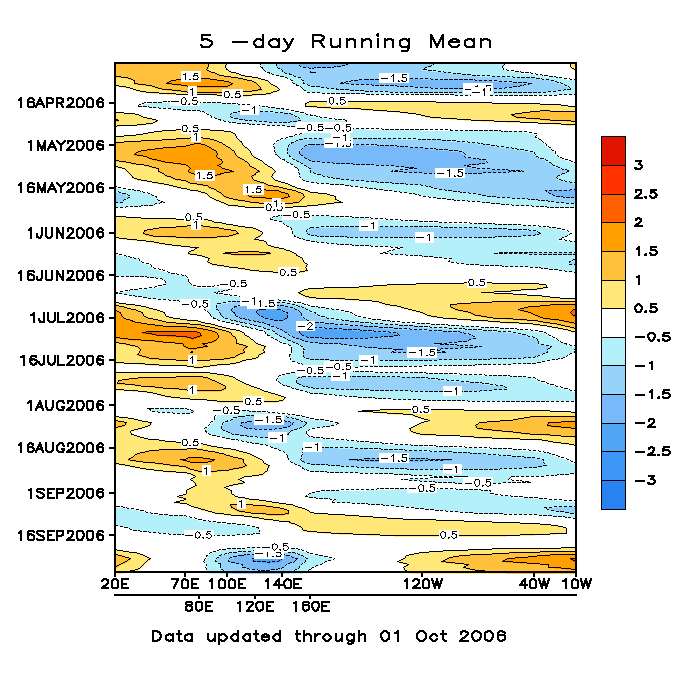
\includegraphics[width=8cm]{Representation/MJO_5-day_running_mean_through_1_Oct_2006}
\centering
\caption{Diagramme de Hovmöller - Émissions des radiations terrestres de longue portée - Source: \textit{U.S. National Oceanic and Atmospheric Administration}}
\end{figure}

En restant à deux dimensions, les séries temporelles condensent les valeurs d'une région pour un paramètre en fonction du temps. Inversement, les cartes spatiales représentent diverses observations à un moment donné. Bien sûr, des données peuvent manquer ou des intervalles de temps peuvent être plus larges et il faut alors recourir à des techniques d'interpolation~\cite{peterson1994spatial}.

La représentation des matrices de corrélation n'est pas dénuée d'intérêts. Tant les notions de \textit{lag} temporel et spatial liés à l'auto-corrélation$^{[\ref{Variation_continue}]}$~\cite{andrienko2003exploratory} que les indicateurs locaux d'association spatiale (LISA)~\cite{anselin1995local} (idée des \textit{Moran's I}$^{[\ref{SpatialProcesses}]}$) qui permettent de s'apercevoir des comportements anormaux du modèle sont des éléments-clefs à la bonne compréhension des données et du problème.

Un autre aspect important est liée à l'analyse spectrale. Ces outils ont beaucoup d'applications et permettent notamment de s'apercevoir des phénomènes de vagues ou d'explorer les structures et motifs dans les données~\cite{chen2007handbook, renshaw1983interpretation}. La décomposition en valeurs propres est attachée aux fonctions orthogonales empiriques (EOF), qui, dans le cas discret, correspondent à l'analyse des composantes principales (PCA). Le cas continu est lié à toute la théorie de Karhunen-Loeve~\cite{jolliffe2002principal}.

\begin{figure}[h]
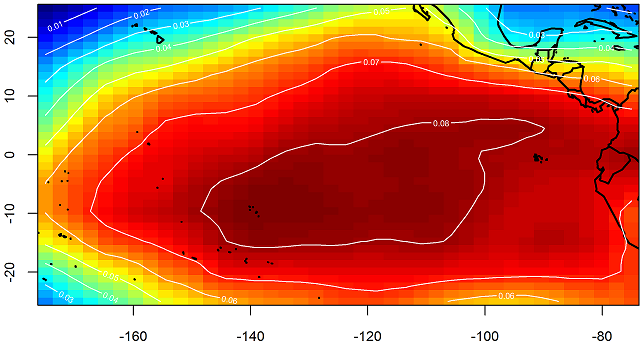
\includegraphics[width=8cm]{Representation/EOF}
\centering
\caption{Répresentation des EOF - Pression au niveau de la mer - Source: \url{http://menugget.blogspot.be/}}
\end{figure}

\subsection{Processus ponctuel}

Naturellement, les concepts liés aux phénomènes spatiaux$^{[\ref{Variation_ponctuelle}]}$ sont étendus pour inclure la notion de temporalité. Mais, on bénéficie de deux nouvelles propriétés, la possibilité de définir une dépendance par rapport au temps et celle de ne pas atteindre un équilibre. On définit alors la fonction d'intensité spatio-temporel $ \lambda(s, t) $ qui représente le nombre d'événements attendus par région par unité de temps. On peut également réaliser une estimation non paramétrique par \textit{kernel smoothing} mais en introduisant une dépendance entre les deux variables~\cite{diggle1985kernel}.

On parle de séparabilité du premier ordre si on est capable de réécrire pour toute région $A$: $ \lambda(s, t) \propto \lambda_{A}(s) \mu_{A}(t) $. Ceci permet de simplifier certains calculs. Il existe également une notion similaire au deuxième moment (et à la stationnarité) et qualifiée de fonction-$K$:

\begin{equation}
    K(u, v) = \lambda^{-1} E[N_{0}(u, v)] \simeq K_{s}(u) K_{t}(v) 
    K(u, v) = \pi u^{2} v + 2 \pi \lambda^{-2} \int_{0}^{v} \int_{0}^{u} \gamma(u', v') u' du' dv'
\end{equation}

Avec $N_{0}(u, v)$ le nombre d'événements dans un disque de rayon $u$ sur un intervalle de temps $[0, v)$ et $\gamma(u, v)$ la densité de covariance~\cite{gabriel2009second}. On peut dès lors employer les processus de Poisson ou de Cox avec le même phénomène que dans le cas spatial, une description naturelle des processus qui ne peuvent être décrits complètement par les variables considérées mais par des interactions stochastiques entre les points.

Enfin, de manière plus générale, on peut s'intéresser aux trajectoires que prennent les points. Historiquement, la première approche proposée a, sans doute, été la définition des mouvements Browniens au travers d'équations différentielles stochastiques~\cite{diggle2013statistical}. Celle-ci demeure très populaire et a été complexifiée en vue d'inclure des notions de dérivées secondes afin de mieux répondre aux problèmes spatiaux. En outre, ces phénomènes ont été également envisagés par l'intermédiaire des VAR, d'équations aux différences ou décrits par des chaînes de Markov~\cite{gelfand2010handbook}.

Librairies R associées: stpp (analyse et simulation de processus ponctuels)~\cite{gabriel2013stpp}, spatstat (fort complet)~\cite{baddeley2016spatial} ou lgcp (pour les processus de Cox)~\cite{lgcp}.

\section{Études antérieures}

Les données spatio-temporelles liées à la mobilité sont très nombreuses. En effet, avec la multiplication des capteurs urbains, l'usage intensif du téléphone portable ou la géolocalisation des applications, il devient plus facile d'être en mesure de mieux déceler et comprendre les comportements humains et leurs déplacements. Bon nombre d'études ont été réalisées sur ce thème.

On peut évidemment s'intéresser à l'aspect principal de la mobilité en tant que déplacement d'une population. La notion capitale attachée est le principe de diffusion qui prévaut dans de nombreux modèles et qui trouve ses origines dans l'écologie. L'idée est que la majorité des gens se déplacement sur de courtes distance mais, avec le temps, ces distances deviennent de plus en plus longues et parfois, on a des voyages sur de fort longues distances~\cite{brockmann2006scaling}.

% Really good: http://cmapspublic.ihmc.us/rid=1GQ6G095M-KLHDV-PSV/Nathan_etal2003Oikos.pdf
Il n'est pas rare de modéliser ce genre de problème par une distribution de Weibull, de Pareto ou exponentielle~\cite{higgins1999predicting}. Ou sous un problème de quantification des motifs tant dans leur changement que dans leur portée. Soit en marquant des individus et en étudiant leur comportement (techniques dites de \textit{Mark-recapture/resighting}). Ou en exploitant un point de vue plus physique, celui de la dualité d'Euler-Lagrange, qui se focalise respectivement sur la population et son évolution sur un large nombre d'individus et sur la caractérisation des déplacements de certains spécimens~\cite{nathan2003methods, southwood2009ecological}.

% Read more carefully https://www.cse.iitb.ac.in/~varsha/allpapers/wireless/adHocModels/mobilty_models_survey.pdf 

Lorsqu'on s'intéresse aux déplacements humains, des aspects plus pratiques rentrent en compte; en effet, nous avons une certaine régularité temporelle et spatiale~\cite{gonzalez2008understanding}. L'un des premiers modèles théoriques développés, outre celui brownien~\cite{einstein1905movement}, fut celui du \textit{Lévy flight} qui donne une distribution à des mouvements aléatoires et permet de représenter des transitions entre deux mouvements browniens~\cite{rhee2011levy, sims2008scaling}. Et on peut alors étudier la dispersion en terme de distances entre les différentes observations~\cite{brockmann2006scaling}. Une extension populaire est celle du \textit{Random waypoint model} dans le cadre du \textit{mobile ad hoc network} (\textit{MANET}) qui semble être un meilleur modèle pour représenter les comportements humains~\cite{camp2002survey}. Enfin, il existe également une approche basée sur des modèles de markov~\cite{bettstetter2001mobility}.

Seulement, toutes ces notions considèrent des mouvements libres où il n'existe aucun obstacle. De surcroît, les humains tendent à optimiser leur trajet. Dans cette optique, des modèles ont été créés~\cite{lee2009slaw}. On peut également mieux prendre en compte les relations sociales ainsi que les cycles journaliers~\cite{cho2011friendship}.

La mobilité peut être observée par divers biais. On peut étudier les déplacements en tant que tels, soit au niveau des taxis qui sont indicateurs de l'activité économique et humaine~\cite{ferreira2013visual}. On peut appliquer des télémétries et de la géolocalisation afin d'en déduire les statistiques liées~\cite{uppoor2014generation}. Une approche plus sociale est également envisageable, on analyse les dynamiques géo-temporelles de l'activité des utilisateurs sur des plateformes de partages de positions telles que: \textit{Twitter}, \textit{Facebook Places}, \textit{Gowalla} et \textit{Foursquare}~\cite{noulas2011empirical, noulas2012tale, hasan2013understanding, cheng2011exploring}. Enfin, analyser les comportements sur base des données de téléphonie mobile est aussi très courant~\cite{becker2013human, de2013unique, ahas2010daily, deville2014dynamic}.

\section{Données}

Depuis 2011, la Commission européenne préconise une démocratisation des données publiques en vue d'une meilleure réutilisation potentielle des services ou produits, de faire face aux challenges sociaux en nous aidant à découvrir des solutions innovantes, d'améliorer l'efficacité des communications dans les administrations et également permettre aux citoyens de prendre part à la vie de la société tout en bénéficiant d'une meilleure transparence pour le gouvernement~\cite{EU-833-2011}.

% http://www.quanturb.com/data.html
Bon nombre de villes ont commencé à mettre en ligne divers ensembles de statistiques et jeux de données. La majorité des grandes villes et métropoles proposent des jeux fort fournis, on peut citer, pour les États-Unis: Chicago, New York, San Francisco, New Orleans, Seattle ou Atlanta et pour l'Europe: le site officiel de l'Union \textit{Data Europa}~\cite{DataEuropa} tente de collecter toutes les données existantes, cependant il est loin d'être complet et on peut alors avoir une vision rapide de nombreuses bases de données à partir de \textit{Open Data Monitor}~\cite{OpenDataMonitor}. La ville de \textit{Köln}, Allemagne semble être un référence en matière de données de transports (\textit{TAPASCologne}). La Chine commence également à produire ses propres données mais ils sont difficiles d'accès pour les non-sinophones.

En Belgique, les données sont moindres malgré les plateformes de \textit{Bruxelles Mobilité}~\cite{BrusselsMobility} et \textit{OpenData Bruxelles}~\cite{OpenDataBruxelles} pour Bruxelles, \textit{Gent stad Data}~\cite{DataGent} pour Gand, \textit{Opendata Antwerpen}~\cite{OpenDataAntwerpen} pour Anvers ainsi que \textit{Data Gov}~\cite{DataGov} et \textit{Open Belgium}~\cite{OpenBelgium} pour la Belgique.

Dans les ensembles de données moins classiques. \textit{Foursquare} fournit une interface indiquant les lieux où se sont rendus les gens~\cite{FourSquare} et des jeux peuvent être trouvés sur internet. On peut également penser à \textit{Twitter} mais certaines restrictions sont appliquées. Pour certaines villes, il existe des données sur les déplacements des taxis et autres véhicules de transports. Enfin, certaines compagnies téléphoniques fournissent des détails de communication des GSM (généralement associé au mot \textit{CDR}). Citons également un jeu de données peu banal, celui du recensement des billets de banque américains en fonction de la commune.
% http://www.nyc.gov/html/tlc/html/about/trip_record_data.shtml

Un outil important dans la simulation du trafic et qui est employé par bon nombres de chercheurs est \textit{Simulation of Urban MObility} (SUMO)~\cite{SUMO2012}. Il a remplacé un ancien simulateur appelé \textit{VanetMobiSim}, extension du programme \textit{CANU Mobility Simulation Environment}. \textit{Geographic Resources Analysis Support System} (GRASS GIS)~\cite{GRASS_GIS_software} est un grand classique dans la gestion et l'analyse de données géospatiales, il permet de modéliser des processus spatio-temporels, produire des images ou de visualiser des données. Dans le même ordre d'idées, il existe les programmes QGIS~\cite{QGIS_software} et ArcGIS (propriétaire)~\cite{ArcGIS_software} qui supportent une visualisation, une édition et une analyse des données spatiales.

% http://cirb.brussels/fr/cirb-smart-city

    % CDR dataset
    % http://aris.me/contents/teaching/data-mining-2015/project/BigDataChallengeData.html
    % https://github.com/rmaestre/d4d-challenge
    % http://crawdad.org/mit/reality/20050701/
    % IMPORTANT -> http://www.pnas.org/content/111/45/15888.full
        % http://www.mdpi.com/2220-9964/1/3/256/htm
        
        % Step by step https://serv.cusp.nyu.edu/~hvo/papers/2016_human_mobility_survey.pdf
        % https://pdfs.semanticscholar.org/312d/98f1c825f4b6f705014bf3860f56e8a51d65.pdf

\section{R packages}

% file:///C:/Users/Youri/Downloads/v63i14%20(1).pdf

De nombreux paquets pour le langage R existent sur le marché afin de répondre à bon nombres de questions liées aux données spatio-temporelles et à leur analyse. Voici une présentation non-exhaustive issue d'un article fort complet sur le sujet~\cite{pebesma2015software}:

\begin{itemize}
    \item SpatioTemporal~\cite{keller2015unified} qui fournit des utilitaires afin d'estimer, prédire et valider des modèles spatio-temporels. Conçu pour l'analyse de pollution atmosphérique et maladie respiratoire.
    \item sp~\cite{sppackage} présente un ensemble de classes et méthodes pour les données spatiales.
    \item gstat~\cite{pebesma2004multivariable} permet de modéliser des problèmes géostatistiques multivariés, de réaliser des prédictions et des simulations. Il supporte les variogrammes spatio-temporels et le \textit{kriging}.
    % Ces deux nécessitent la fonction de covariance qui ne marche pas pour les grands datasets
    \item spacetime~\cite{pebesma2012spacetime} pour manipuler et explorer des données.
    \item RandomFields~\cite{schlather2015analysis} permet d'estimer les hyper-paramètres des champs aléatoire Gaussiens sur base du maximum de vraisemblance ou des moindres carrés.
    \item stpp~\cite{gabriel2013stpp} afin d'analyser, simuler and montrer des motifs des points spatio-temporels.
    \item spatstat~\cite{baddeley2016spatial} est fort complète pour étudier les processus ponctuels et propose tous les outils possibles et imaginables dont vous pourriez avoir besoin.
    \item spBayes~\cite{finley2007spbayes} pour les processus ponctuels univariés et multivariés sous les modèles bayésiens.
    \item spate~\cite{sigrist2015spate} pour modéliser par le biais des équations aux dérivées partielles stochastiques.
\end{itemize}

%spdep (Bivand 2009)
%ncf (Bjornstad 2009)
%nlme (Pinheiro et al. 2008)

%BACCO - Bayesian analysis of computer code software
%tgp - Treed Gaussian processes
%DiceDesign, DiceEval, DiceKriging, DiceOptim - metamodeling packages of the Dice Consortium

\section{Conclusion}

Vous l'aurez compris, l'analyse de données spatio-temporel
s est un incroyablement vaste domaine qui trouve ses origines dans les années 60. Malgré toutes ces années d'étude, il reste bon nombre de problèmes ouverts. Les enjeux liés à cette problématique sont immenses et offrent des aspects très diversifiés. La recherche de solutions à ces problèmes est encore activement sujet à études et est porteuse d'une diversité phénoménale tant dans la manière d'envisager et d'approcher ces notions que dans leur réalisation sur le terrain. Et ce, en dépit de l'avènement des ordinateurs et de leur augmentation en puissance de calcul qui a permis de développer de nouveaux modèles toujours plus complexes.

Ils demeurent de nombreux concepts clefs mal perçus même si les études sur les déplacements des populations, et des humains plus spécifiquement, se sont multipliés. Les applications sont innombrables, tant au niveau de la physique, de l'économie ou de l'urbanisme. C'est un véritable bouleversement que propose l'analyse des données spatio-temporelles. Par ailleurs, notre monde devient de plus en plus connecté et les données affluent dans tous les sens et ne demandent qu'à être analysées. Nous pouvons espérer, par cette quantité, mieux comprendre les dynamiques sous-jacentes et les impacts sur notre vie au quotidien.
